\graphicspath{{figures/results/}}
\chapter{Results}
The results presented are both training and testing results from the two solutions. Both the image classification bound occlusion detection and the multi-class object detection bound occlusion detection are trained and tested on the 60 seconds video with three fish.

It is trained on annotated data of around 200 different occlusions in total and annotated "no occlusions".
%The results presented are made by labelling all occlusions happening in the data. This covers the two videos provided by Loligo Systems which include three and five fish, each just about one minute long. The labelling is done by marking the point in which an occlusion is spotted, with skeletons drawn on each image. The frames of the video in which no occlusions occur does not have any labelling.
%
\section{Image Classification}
The image classification is trained for 15 epochs.
\begin{figure}[H]
	\centering
	\begin{subfigure}{0.48\textwidth}
		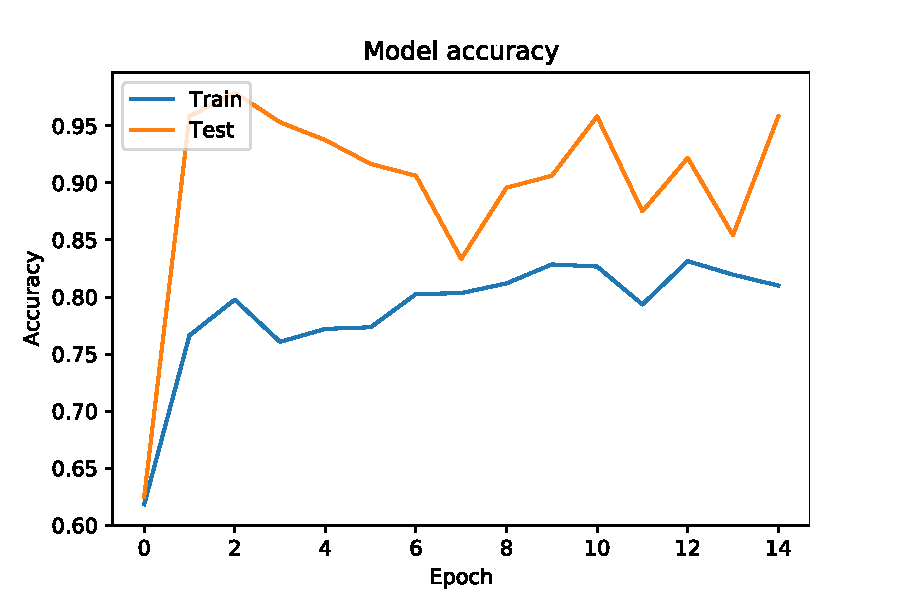
\includegraphics[width=\textwidth]{model_acc_15epoch}
		\caption{The image classification accuracy for both training and testing}
		\label{fig:img_acc-15}
	\end{subfigure}
	\begin{subfigure}{0.48\textwidth}
		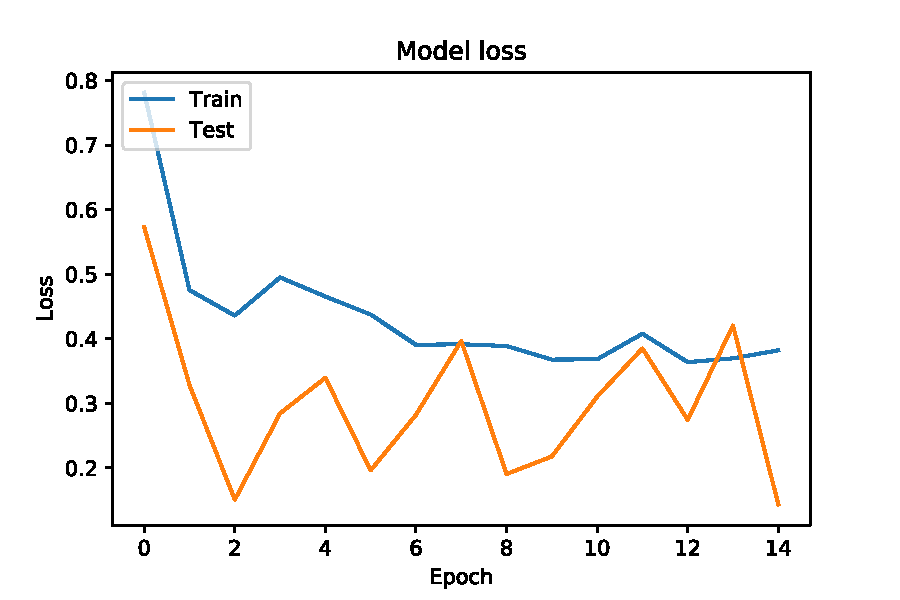
\includegraphics[width=\textwidth]{model_loss_15epoch}
		\caption{The image classification loss for both training and testing}
		\label{fig:img_loss-15}
	\end{subfigure}
\caption{Heading}
\label{fig:img_class-15ep}
\end{figure}
The model here achieves: 
\begin{table}[H]
	\centering
	\caption{Results achieved with 15 epochs.}
	\begin{tabular}{|l|l|}
		\hline
		Loss                & 0.4841 \\\rowcolor{lightGrey}\hline
		Accuracy            & 0.7738 \\ \hline
		Validation Loss     & 0.2487 \\\rowcolor{lightGrey}\hline
		Validation Accuracy & 0.9318\\ \hline
	\end{tabular}
\label{tab:img_class_15ep}
\end{table}

The model is also trained for 100 epochs, the results of this is shown in \autoref{fig:img_class-100ep} and \autoref{tab:img_class_100ep}.
\begin{figure}[H]
	\centering
	\begin{subfigure}{0.48\textwidth}
		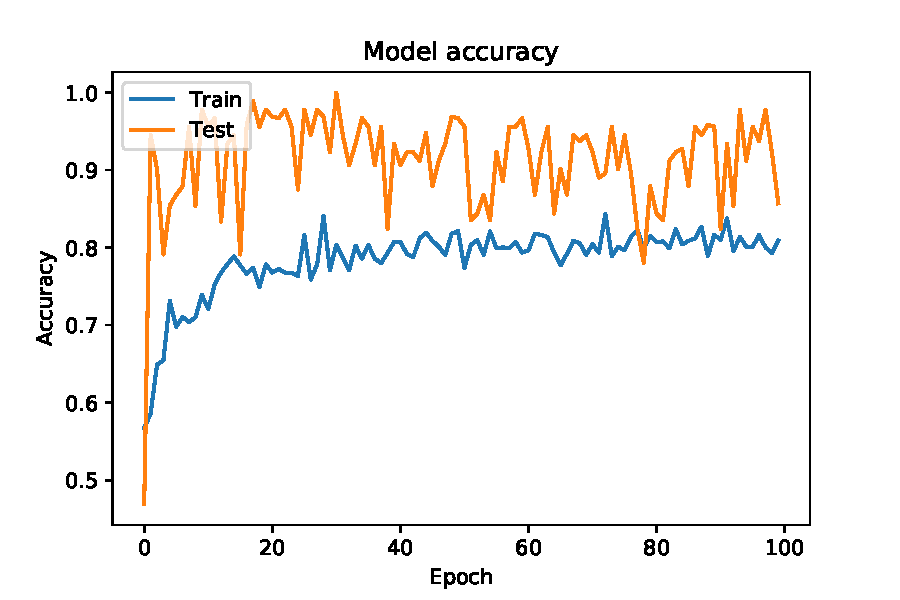
\includegraphics[width=\textwidth]{model_acc_100epoch}
		\caption{The image classification accuracy for both training and testing}
		\label{fig:img_acc-100}
	\end{subfigure}
	\begin{subfigure}{0.48\textwidth}
		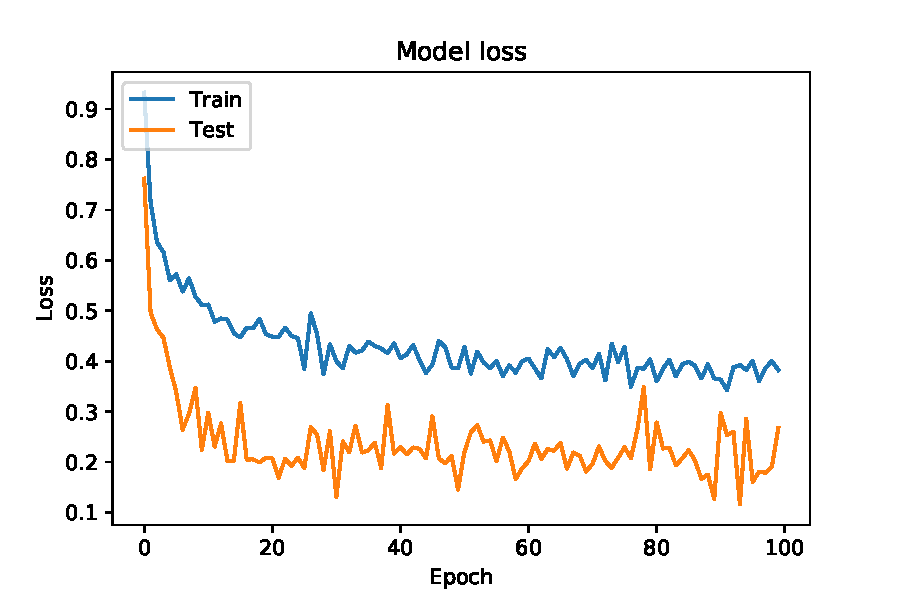
\includegraphics[width=\textwidth]{model_loss_100epoch}
		\caption{The image classification loss for both training and testing}
		\label{fig:img_loss-100}
	\end{subfigure}
\caption{heading}
\label{fig:img_class-100ep}
\end{figure}

\begin{table}[H]
	\centering
	\caption{Results achieved with 100 epochs.}
	\begin{tabular}{|l|l|}
		\hline
		Loss                & 0.3831 \\\rowcolor{lightGrey}\hline
		Accuracy            & 0.8075 \\ \hline
		Validation Loss     & 0.2680 \\\rowcolor{lightGrey}\hline
		Validation Accuracy & 0.8571\\ \hline
	\end{tabular}
	\label{tab:img_class_100ep}
\end{table}

\section{Object Detection}
The multi class object detection solution is also presented with two different amounts of training. This is for 42 epochs and for 152 epochs.

\subsection{42 Epochs}
When trained for 42 epochs, the training accuracy is as shown in the following figures:
\begin{figure}[H]
	\centering
	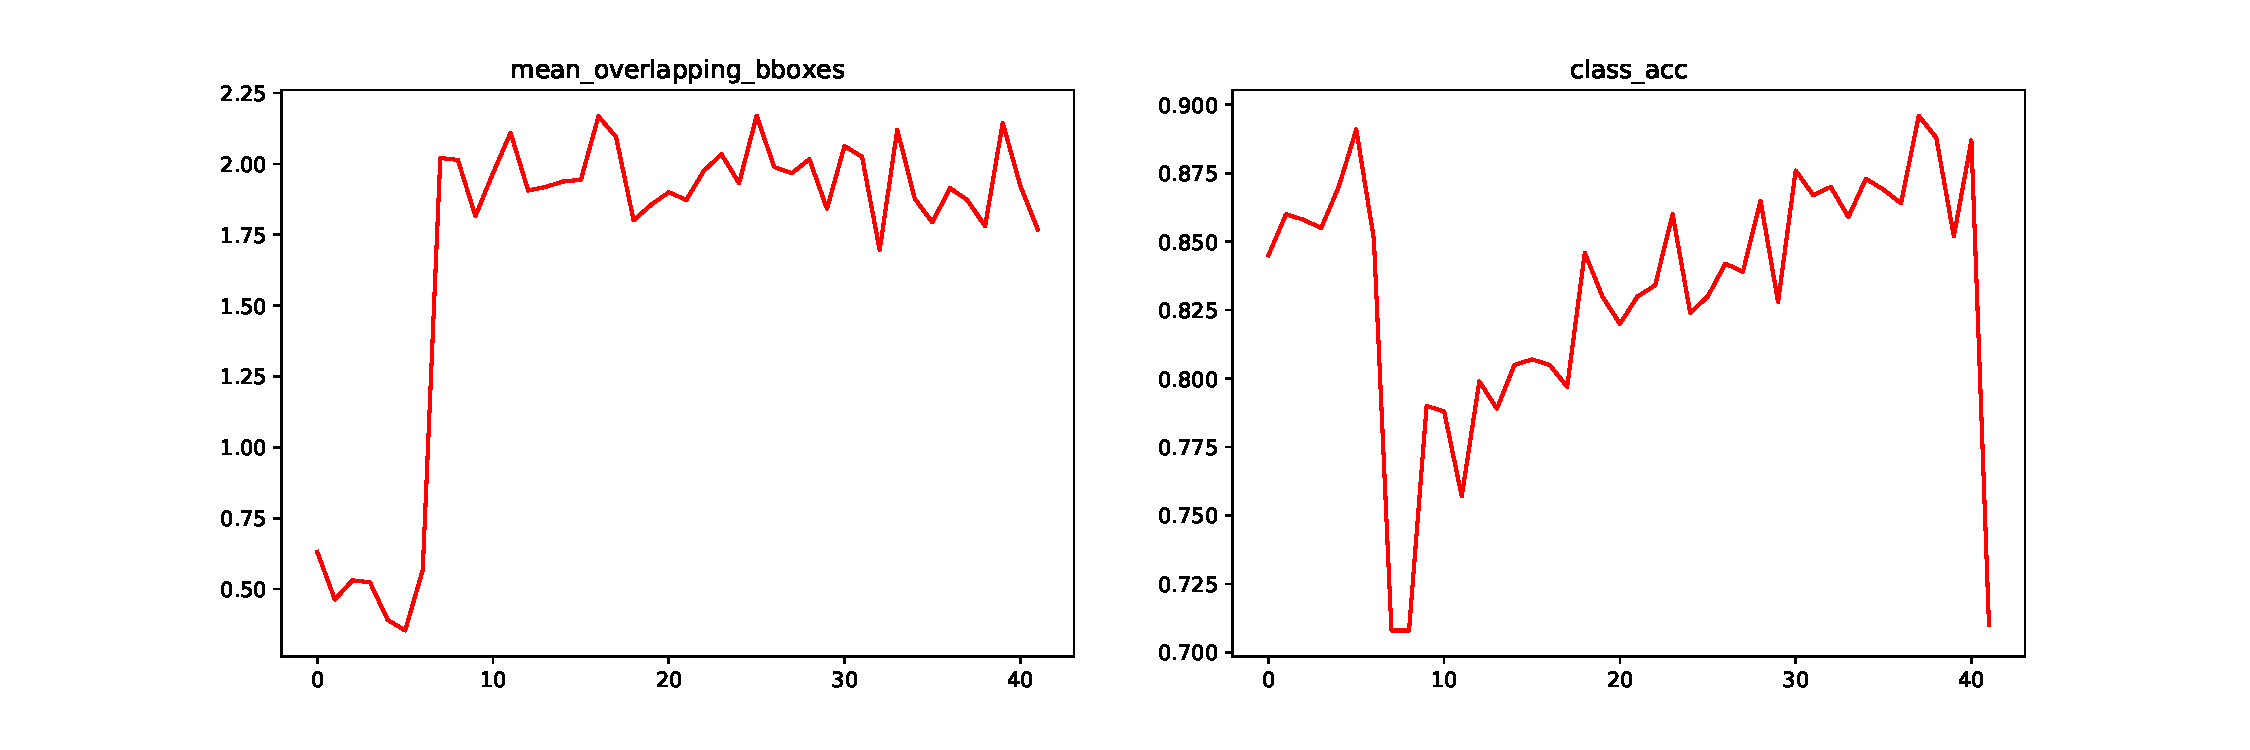
\includegraphics[width=\textwidth]{acc-42}
	\caption{Accuracy}
	\label{fig:acc-42}
\end{figure}
\begin{figure}[H]
	\centering
	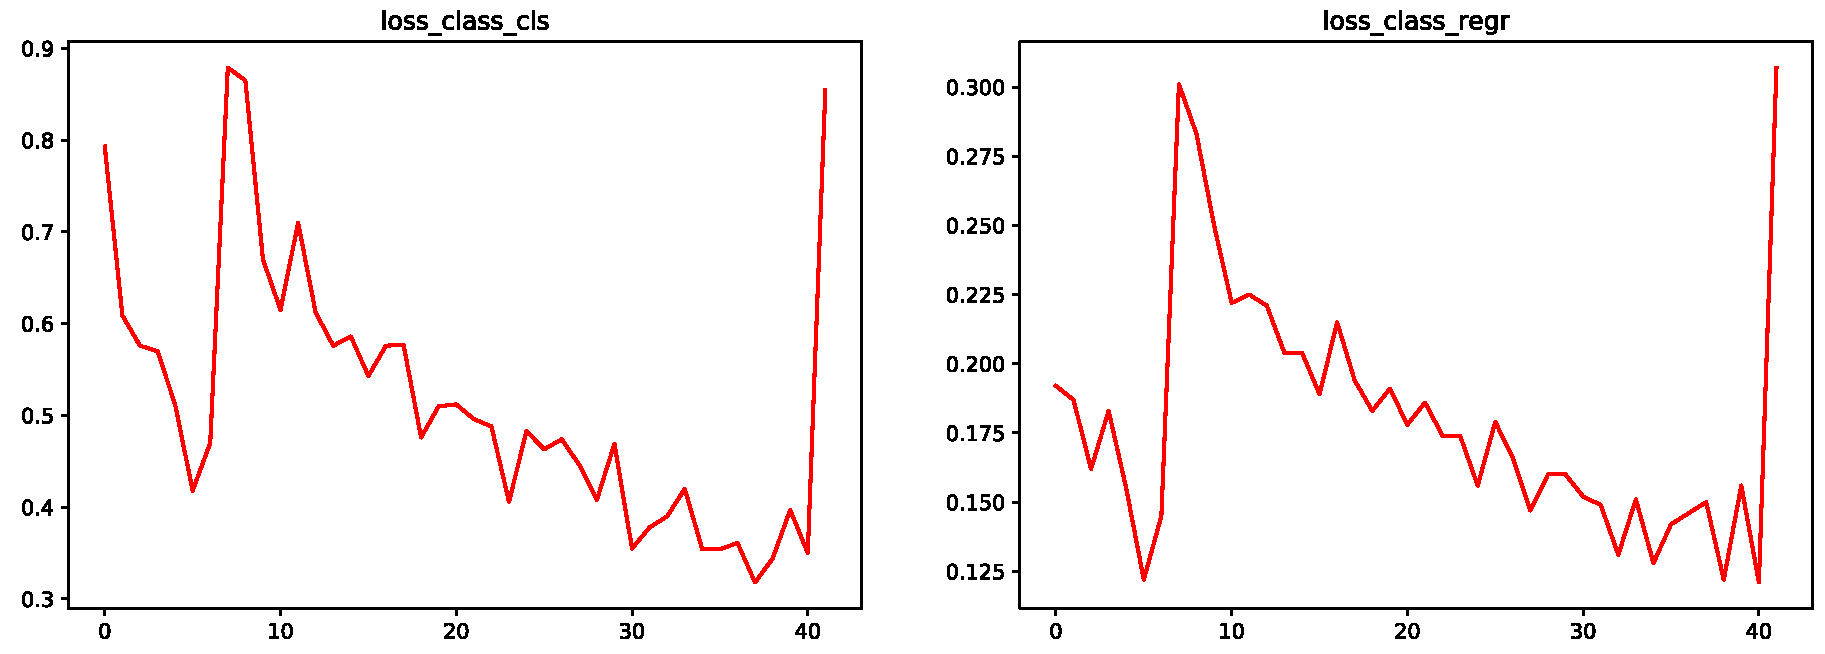
\includegraphics[width=\textwidth]{loss_class-42}
	\caption{Loss Class - classification and bbox regression}
	\label{fig:loss_class-42}
\end{figure}
\begin{figure}[H]
	\centering
	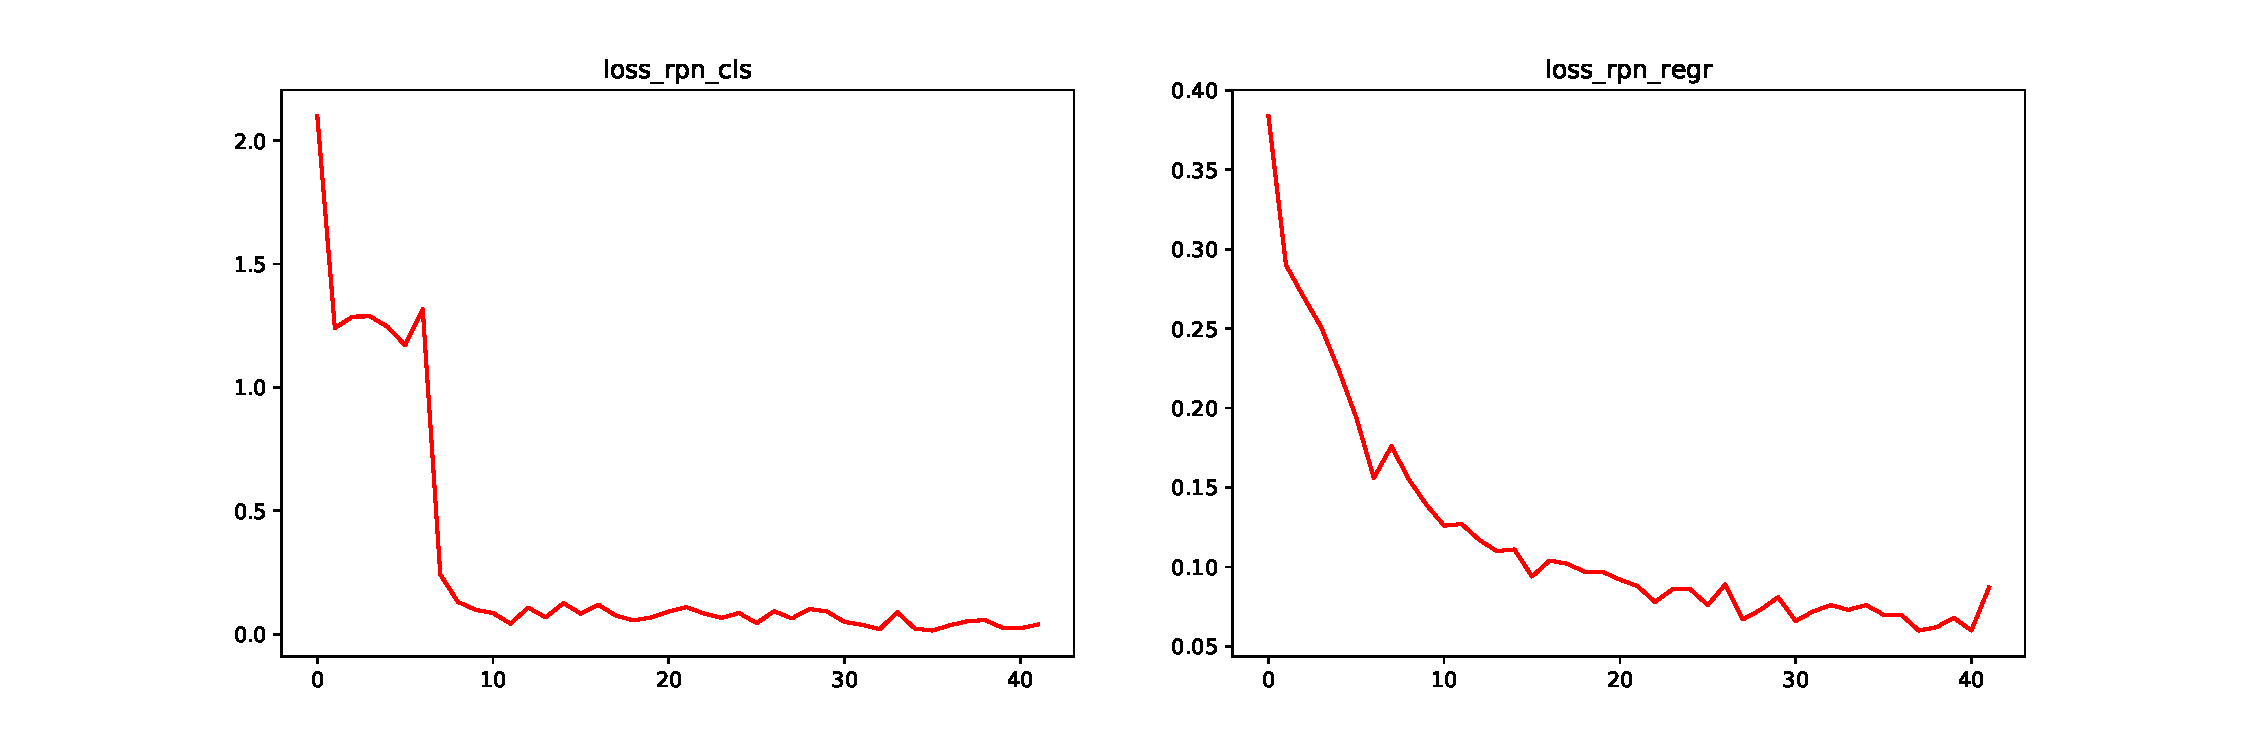
\includegraphics[width=\textwidth]{loss_rpn-42}
	\caption{Loss Region Proposal Network - classification and bbox regression}
	\label{fig:loss_rpn-42}
\end{figure}
\begin{figure}[H]
	\centering
	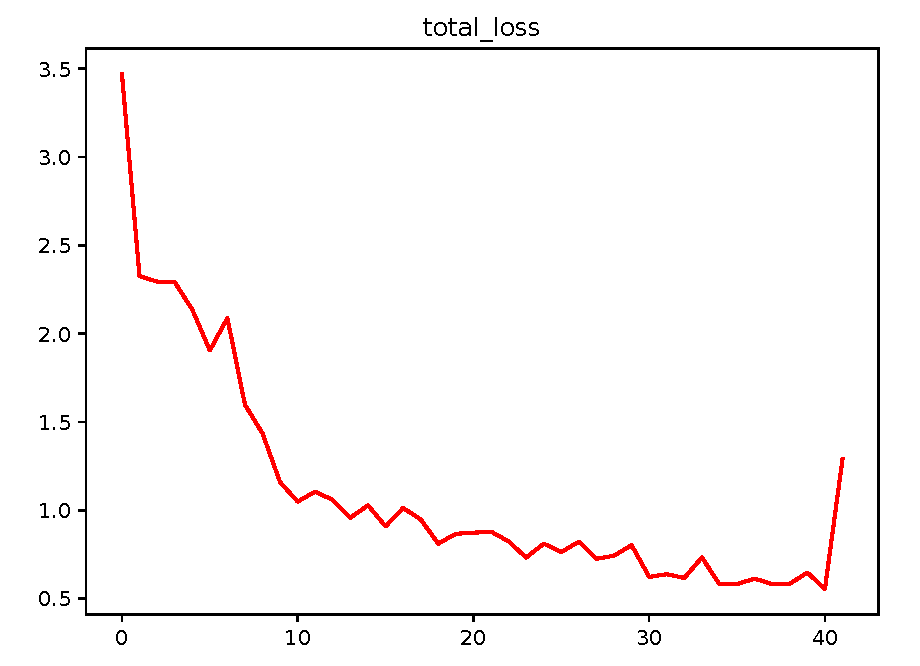
\includegraphics[width=0.85\textwidth]{total_loss-42}
	\caption{Total loss}
	\label{fig:total_loss-42}
\end{figure}

When testing with this result, the test was stopped due to poor performance.

\subsection{135 Epochs}
\begin{figure}[H]
	\centering
	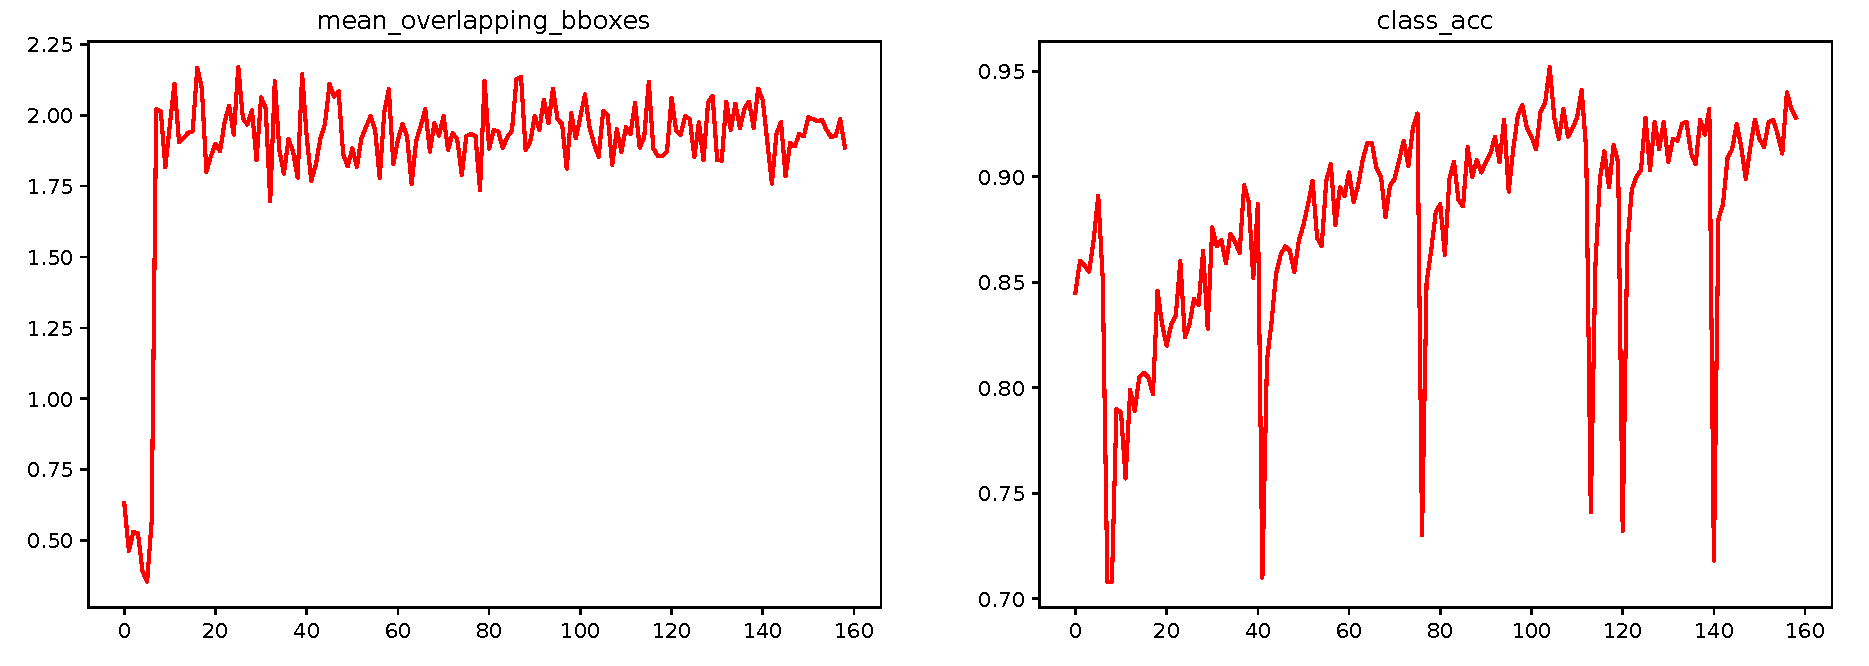
\includegraphics[width=\textwidth]{acc-152}
	\caption{Accuracy}
	\label{fig:}
\end{figure}
\begin{figure}[H]
	\centering
	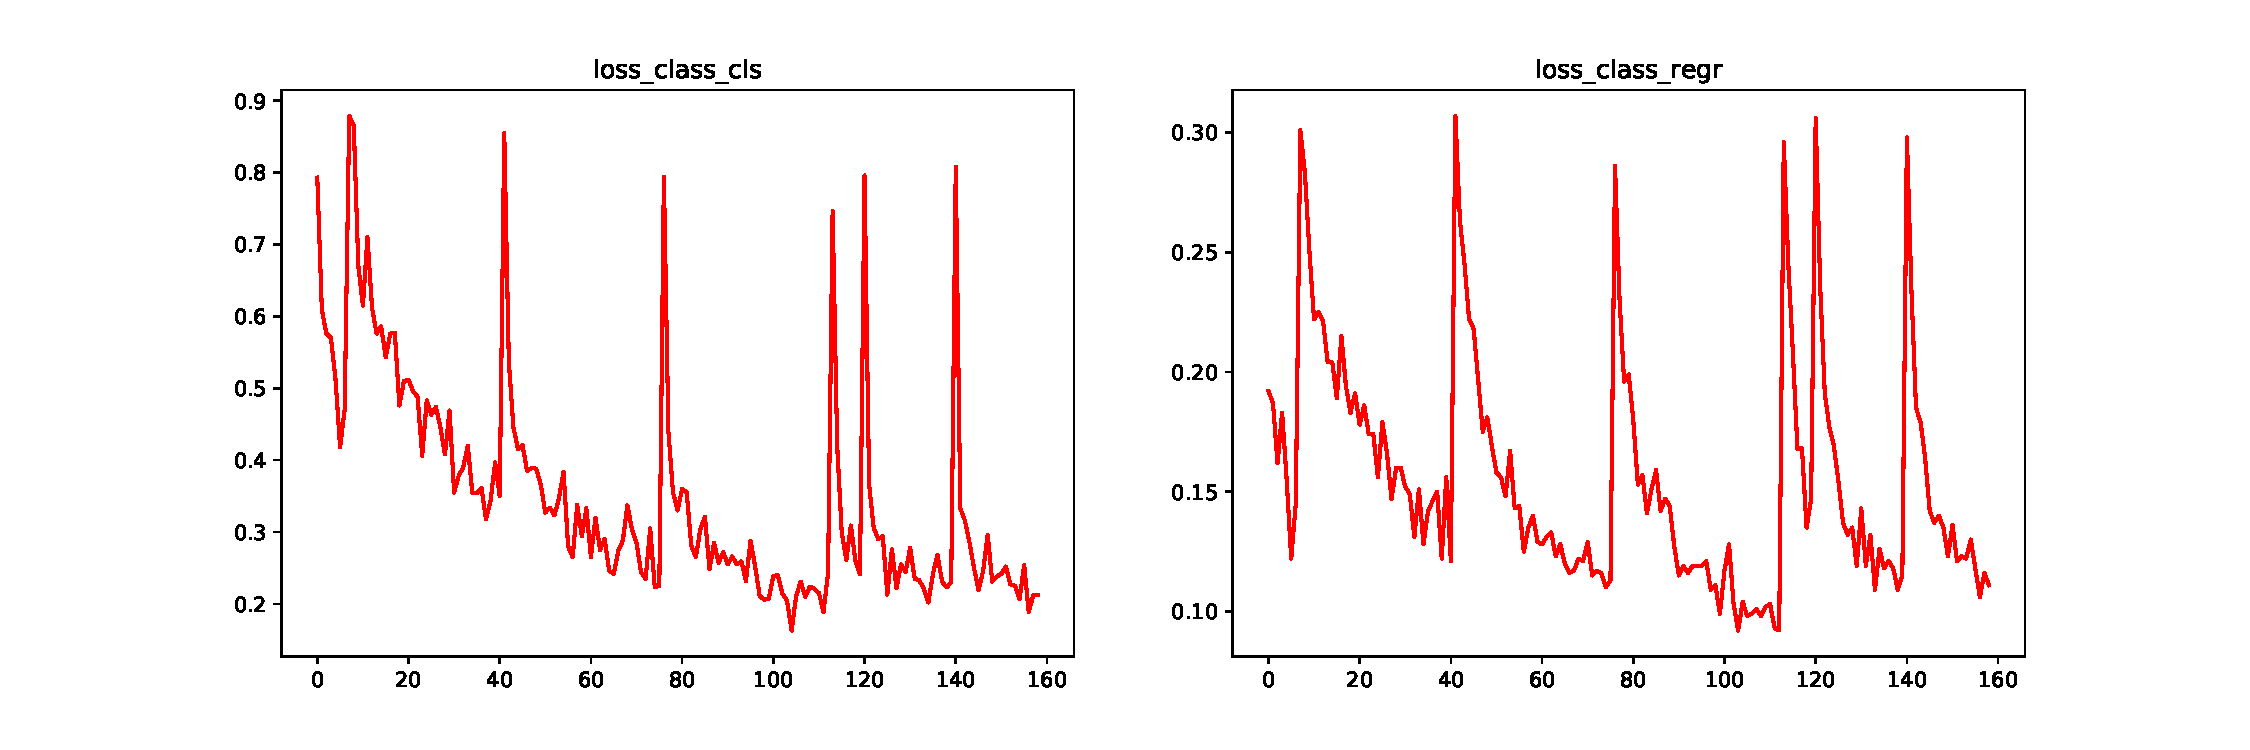
\includegraphics[width=\textwidth]{loss_class-152}
	\caption{Loss Class - classification and bbox regression}
	\label{fig:}
\end{figure}
\begin{figure}[H]
	\centering
	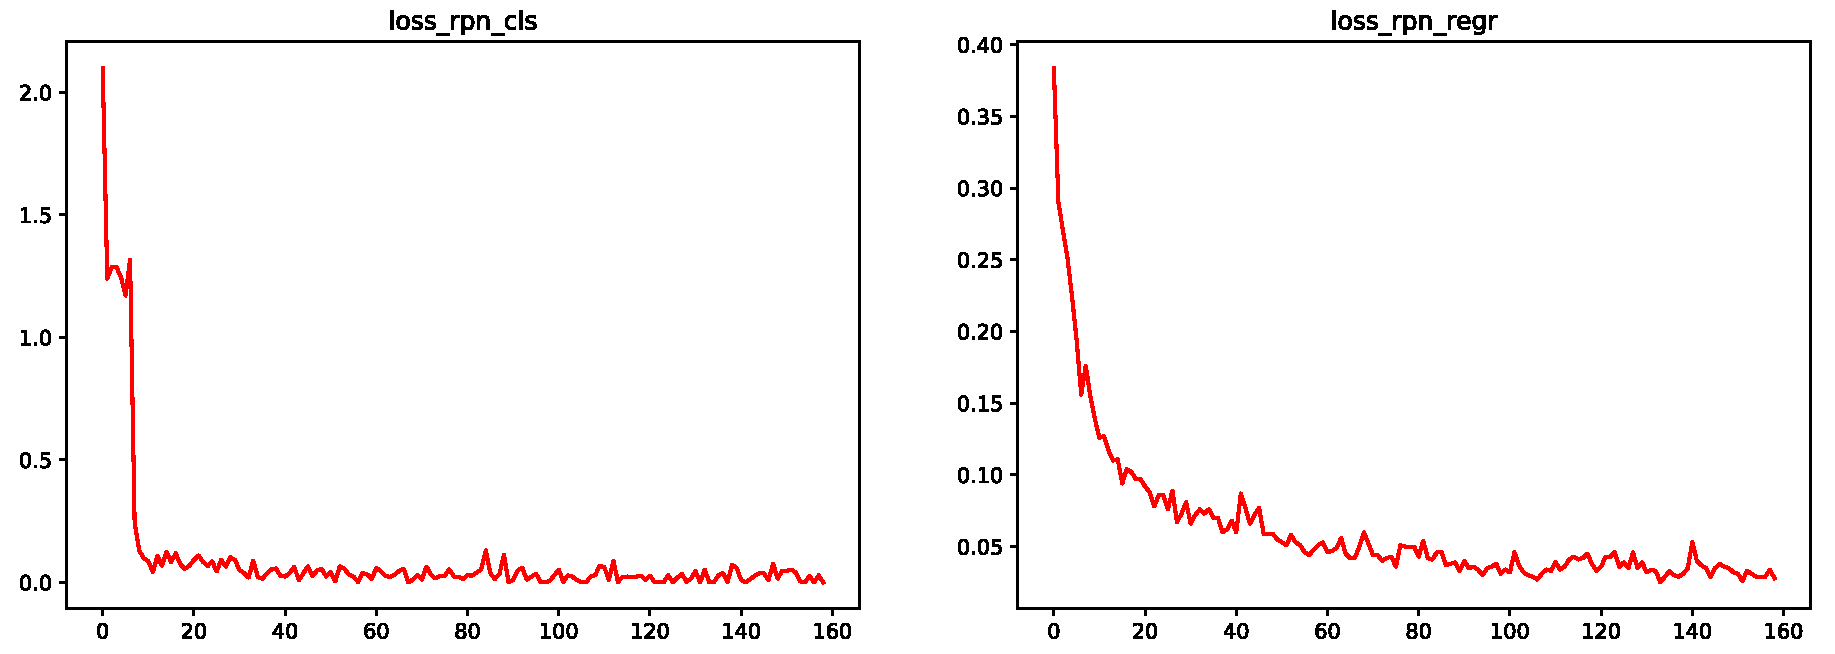
\includegraphics[width=\textwidth]{loss_rpn-152}
	\caption{Loss Region Proposal Network - classification and bbox regression}
	\label{fig:}
\end{figure}
\begin{figure}[H]
	\centering
	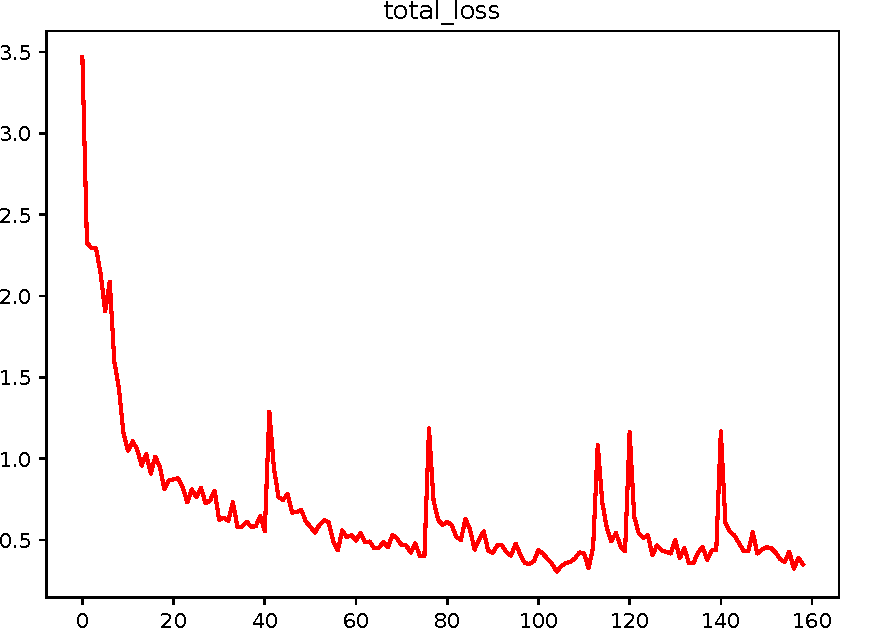
\includegraphics[width=0.7\textwidth]{total_loss-152}
	\caption{Total loss}
	\label{fig:}
\end{figure}


\section{Testing}
The training and testing split is done with $85\%,15\%$ for training and testing. With this the solution reaches a \gls{map} of $66.8\%$.

\autoref{fig:T-det}, \ref{fig:not-det}, and \ref{fig:no-occl-det} show plots of predictions of three random testing frames, with predictions and bounding box regressions. The predictions and the accuracy is written in the image caption. Only detections with a confidence above $70\%$ are accepted.\\

The average precision of the different classes are shown in \autoref{tab:class-pred}.


\begin{table}[H]
	\centering
	\caption{Average precisions of the different occlusion types}
	\label{tab:class-pred}
	\begin{tabular}{ll}
		\textbf{Occlusion Type} & \textbf{Average Precision} \\\rowcolor{lightGrey}\hline
		T Shape                 & 74.6\%                     \\
		V Shape                 & 53.9\%                     \\\rowcolor{lightGrey}
		On Top                  & 100\%                      \\
		Cross                   & 78.2\%                     \\\rowcolor{lightGrey}
		Elongation              & 91.9\%                     \\
		Other                   & 37.6\%                     \\\rowcolor{lightGrey}
		No Occlusion            & 34.6\%                    
	\end{tabular}
\end{table}

\begin{figure}[H]
	\centering
	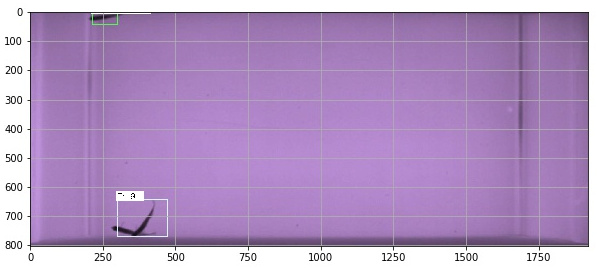
\includegraphics[width=\textwidth]{prediction-frame596}
	\caption{Detection of the T-shape is with a confidence of $91.37\%$ and of no occlusion with $99.48\%$}
	\label{fig:T-det}
\end{figure}
\begin{figure}[H]
	\centering
	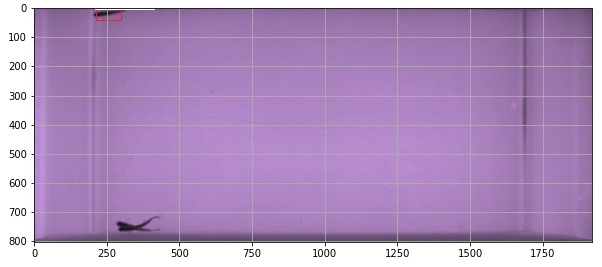
\includegraphics[width=\textwidth]{prediction-frame601}
	\caption{Only detection of no occlusion with confidence of $99.43\%$}
	\label{fig:not-det}
\end{figure}
\begin{figure}[H]
	\centering
	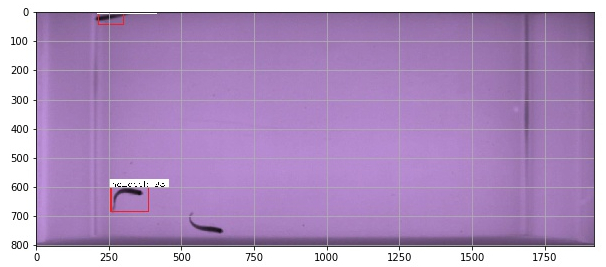
\includegraphics[width=\textwidth]{prediction-frame1092}
	\caption{Two detections of no occlusions with confidence of $99.48\%$ and $98.73\%$}
	\label{fig:no-occl-det}
\end{figure}